\chapter{الگوریتم بهینه‌سازی REMARK}
عرضه و تقاضا دو عامل ضروری تحلیل بازار را تشکیل می‌دهند. مفاهیم اساسی این نظریه‌ی اقتصادی در ادامه به اختصار بررسی شده است.

\section{تقاضا}
بر اساس نظریه مرسوم اقتصاد، منحنی تقاضا، مکان هندسی مجموعه نقاطی است، که یک فرد برای به دست آوردن کالا یا خدماتی با قیمت‌های مختلف حاضر به پرداخت پول است. این مکان هندسی با فرض آن است که تمامی شرایط  ثابت نگه داشته شده است. 
 وقتی قیمت یک کالا کاهش می‌یابد، مردم تقاضای بیشتری را نشان می دهند، مشروط بر اینکه همه‌ی شرایط برابر باشد. به طور مشابه، هر چه قیمت بالاتر باشد، مقدار کمتری تقاضا می‌شود. مقدار تقاضا با توجه به منحنی تقاضا نسبت به قیمت حساس است. شکل \ref{fig:demand} نمونه ای از منحنی تقاضا را نشان می دهد که نشان می دهد چگونه تقاضا ($Q$) با قیمت ($P$) تغییر می‌کند. شیب منحنی بر حساسیت تقاضا نسبت به تغییر قیمت تأثیر می گذارد.
 
 \begin{figure}[H]
 	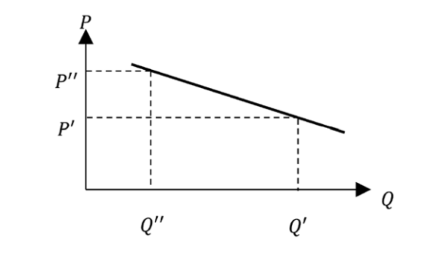
\includegraphics[width=6cm]{../Figure/introduction/demand.png}
 	\centering
 	\caption{قضیه اساسی تقاضا
 		\cite{Nobahari2022}}
 	\label{fig:demand}
 \end{figure}

لازم به ذکر است که مقدار تقاضا علاوه بر قیمت به عوامل برون زا بستگی دارد. این عوامل را می توان اندازه بازار، انتظار افزایش قیمت و غیره نام برد. عوامل برون زا باعث تغییر در برنامه تقاضا مانند شکل \ref{fig:demand_shift} می شود.

 \begin{figure}[H]
	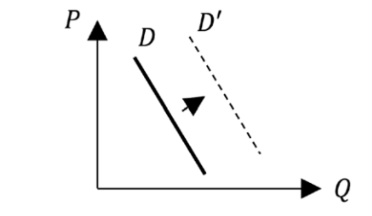
\includegraphics[width=5cm]{../Figure/introduction/demand_shift.png}
	\centering
	\caption{تغییر در برنامه تقاضا}
	\label{fig:demand_shift}
\end{figure}

\section{عرضه}

مکان هندسی عرضه، مجموعه‌ای از مقدار فرضی کالایی است که عرضه‌کنندگان در هر قیمت عرضه می‌کنند. هنگام برخورد با املاک و مستغلات، سه مفهوم عمده در عرضه وجود دارد: عرضه کل بلندمدت، عرضه کل کوتاه‌مدت و ساخت‌و‌ساز جدید. شکل
\ref{fig:supply_short_term}
  عرضه کل کوتاه‌مدت را نشان می‌دهد. عرضه کل کوتاه‌مدت به کل موجودی یک بازار در یک زمان معین اشاره می‌کند. سهام املاک و مستغلات به‌دلیل زمان مورد نیاز برای ساخت املاک جدید، در کوتاه‌مدت  ثابت است، که به آن تاخیر ساخت‌و‌ساز می‌گویند. شکل
  \ref{fig:supply_long_term}
   عرضه کل بلندمدت را نشان می دهد که به رابطه‌ی بین مقادیر عرضه شده و قیمت های بلندمدت اشاره دارد. با این وجود، هنگام تجزیه و تحلیل بازارهای املاک و مستغلات، مهمترین مفهوم در عرضه، ساخت‌و‌ساز جدید است. به دلیل اینکه عمر دارایی مستغلات طولانی است، برنامه ساخت و ساز جدید از قانون اساسی عرضه پیروی می‌کند. قانون اساسی عرضه  می‌گوید که، هر چه قیمت ملک بالاتر باشد، نرخ ساخت و ساز بالاتر است.

\begin{figure}[H]
	\centering
	\subfloat[]{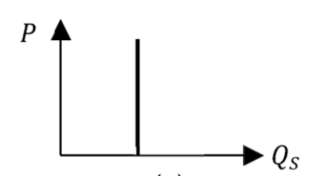
\includegraphics[width=.35\linewidth]{../Figure/introduction/supply_short_term.png}\label{fig:supply_short_term}}
	\subfloat[]{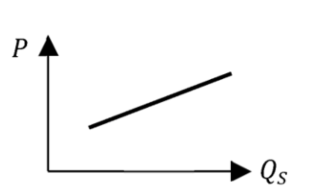
\includegraphics[width=.35\linewidth]{../Figure/introduction/supply_long_term.png}\label{fig:supply_long_term}}
	\caption{قضیه اساسی تقاضا}
\end{figure}

\section{تنظیم قیمت}

قیمت بازار از طریق تعامل عرضه‌کنندگان (فروشندگان) و تقاضاکنندگان (خریداران) در بازار مشخص می‌شود.
مطابق شکل 5، فرض کنید که قیمت زیر نقطه تعادل در $P_1$ است. در این سطح، مقدار تقاضای $Q_{D_1}$، بیشتر از مقدار عرضه شده $Q_{S_1}$ است. این امر باعث افزایش قیمت می‌شود به طوری که تعدادی از خریداران از بازار خارج می‌شوند و تعدادی فروشنده جدید وارد بازار می‌شوند. هنگامی که قیمت به نقطه تعادل $P^*$ رسید که در آن $Q_D = Q_S$، خریداران انگیزه‌ای برای افزایش قیمت نخواهند داشت. هنگامی که قیمت بالاتر از نقطه تعادل در $P_2$ باشد، مقدار $Q_{D_2}$ تقاضا شده، کوچکتر از مقدار عرضه شده $Q_{S_2}$ است و فروشندگان برای جذب خریداران انگیزه برای کاهش قیمت خواهند داشت. قیمت تا رسیدن به نقطه تعادل کاهش می‌یابد که در آن$Q_D = Q_S$ و فروشندگان انگیزه‌ای برای کاهش بیشتر قیمت نخواهند داشت.

 \begin{figure}[H]
	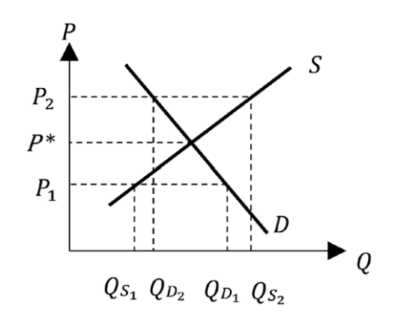
\includegraphics[width=5cm]{../Figure/introduction/market_price.png}
	\centering
	\caption{تعیین قیمت در بازار}
	\label{fig:market_price}
\end{figure}


